% Guard: macros.tex is \input both by main.tex (after the packages it needs,
% e.g. amsmath for \DeclareMathOperator) and by individual section files so
% they remain compilable on their own. Loading it twice would redefine every
% \newcommand and abort, so the second and later loads are no-ops.
\ifdefined\PQRmacrosloaded\endinput\fi
\let\PQRmacrosloaded\relax

% --- 0. revision marking ---
% Text added to Section 2 during the current revision is wrapped in \added{...}
% so the advisors can see at a glance what is new. Redefine to \relax to print
% the paper without the marking.
\newcommand{\added}[1]{\textcolor{blue}{#1}}
\long\def\added#1{\begingroup\color{blue}#1\endgroup}  % \long: may span paragraphs


% --- A. operator-style score and function names ---
\newcommand{\HD}{\mathit{HD}}                        % histogram distance; use \HD_\gamma
\newcommand{\Attr}{\mathit{Attr}}                    % attribute set of a schema
\newcommand{\Attrs}{\mathit{Attrs}}                  % attribute set argument
% Abbreviated in MATH only; the prose still spells the names out in full.
% Spelling them out inside formulas makes displayed equations far too wide
% for a two-column layout (the product-rule step below overflowed by 200pt).
\newcommand{\Use}{\mathit{Use}}
\newcommand{\Cov}{\mathit{Cov}}
\newcommand{\Rep}{\mathit{Rep}}
\newcommand{\DivS}{\mathit{Div}}
\newcommand{\TVD}{\mathit{TVD}}
\newcommand{\GS}{\mathit{GS}}                        % global sensitivity
\DeclareMathOperator{\Dom}{Dom}
\DeclareMathOperator{\Lap}{Laplace}

% --- B. core objects ---
\newcommand{\Qone}{Q_1}
\newcommand{\Qtwo}{Q_2}
\newcommand{\pD}{p(D)}
\newcommand{\views}{\mathcal{P}}
\newcommand{\hist}[2]{H_{#1,#2}}                     % \hist{\Qone(\pD)}{A}
\newcommand{\dhist}{\Delta H}
\newcommand{\nhist}{\widetilde{\Delta H}}            % the released noisy object

% --- C. privacy budget and parameters ---
\newcommand{\eps}{\epsilon}
\newcommand{\epsP}{\epsilon_P}
\newcommand{\epsS}{\epsilon_S}
\newcommand{\epsH}{\epsilon_H}
\newcommand{\gammaref}{\gamma_{\mathrm{ref}}}
\newcommand{\gammaeval}{\gamma_{\mathrm{eval}}}
\newcommand{\taumax}{\tau_{\max}}

% --- D. mechanisms ---
\newcommand{\ExpMech}{\textsc{ExpMech}}
\newcommand{\OneShotTop}[1]{\textsc{OneShotTop-}#1}
\newcommand{\AdaptiveTau}{\textsc{AdaptiveTau}}
% --- E. experiment baselines (used in sections/experiments.tex) ---
\newcommand{\Bone}{\ensuremath{\mathsf{B1}}}
\newcommand{\Btwo}{\ensuremath{\mathsf{B2}}}
\newcommand{\Bthree}{\ensuremath{\mathsf{B3}}}

\section{Algorithm}\label{sec:solution}

\subsection{Overview}
\label{subsec:algorithm-overview}

The algorithm follows the model introduced in Section~\ref{sec:model}.
It first privately selects a small set of useful predicate views, then constructs explanation candidates by pairing selected views with attributes, and finally privately selects and releases the top-$k$ histogram explanations.
This structure mirrors recent differentially private explanation frameworks, which separate the definition of explanation quality from the design of low-sensitivity private selection mechanisms \cite{TaoGMR22}.

Designing a practical algorithm for private query-difference explanations requires addressing two central challenges.
First, generating all possible views is infeasible because the space of predicate-defined subpopulations is combinatorial.
We therefore work with a candidate set $\mathcal{P}$ of predicate-based views, as is common in explanation and subgroup-discovery frameworks \cite{FEDEX,ICDE23}.
Second, the ideal utility function from Section~\ref{sec:explanation-quality} has high sensitivity and may be expensive to optimize.
We therefore introduce low-sensitivity proxy measures that capture the same conceptual goals: Histogram Distance for interestingness, Usefulness for representativeness and coverage, and DiversityScore for diversity.

Four refinements distinguish the algorithm presented here, each motivated by a specific failure of the direct formulation and each validated experimentally in Section~\ref{sec:experiments}:
\begin{enumerate}
  \item \textbf{Smoothed Histogram Distance} (Section~\ref{subsubsec:histogram-distance}). The unsmoothed score is a ratio whose global sensitivity is dictated by arbitrarily small histogram bins, even though almost all candidates rest on large ones. Smoothing the denominator by a public constant $\gamma$ yields a provably tighter bound and is the single change responsible for most of the empirical improvement.
  \item \textbf{Graded diversity} (Section~\ref{subsubsec:diversity-score}), which penalises the $j$-th reuse of an attribute by $\lambda^{j-1}$ rather than a flat $\lambda$, together with an order-independent set-level objective that makes Definition~\ref{def:setobj} well posed and monotone submodular.
  \item \textbf{Budget-derived $\tau$ and $\gamma$} (Section~\ref{subsubsec:adaptive-params}), following the annealing strategy of AIM~\cite{McKennaMSM22}: both are functions of the \emph{public} privacy accountant, so adapting them costs no privacy budget.
  \item \textbf{Smoothed Representativeness} (Section~\ref{subsubsec:view-usefulness}). The same remedy applied to the view-selection score, for the same reason: it too is built from a ratio whose denominator is a view size. Without it the sensitivity constant of View Usefulness does not stabilise as the database grows.
\end{enumerate}

\begin{figure*}[t]
\centering
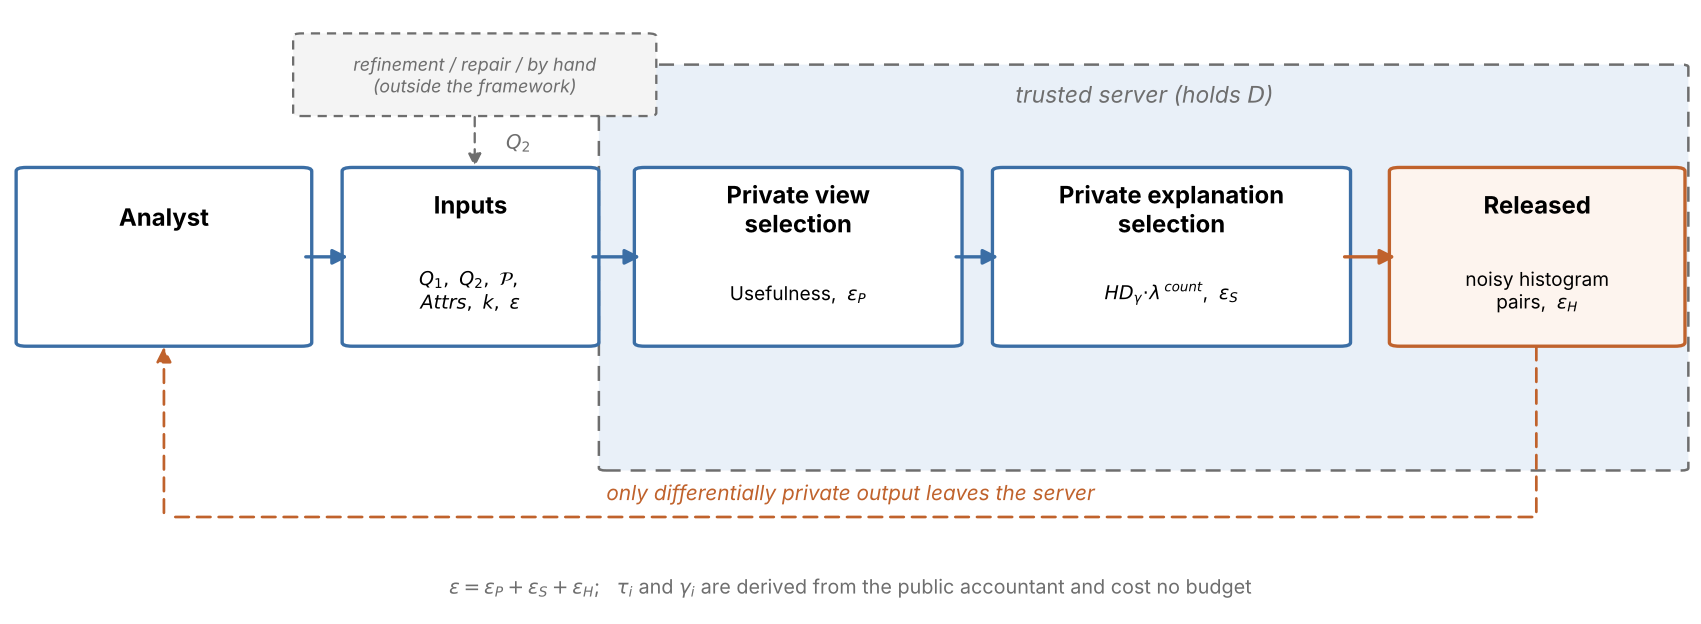
\includegraphics[width=\linewidth]{figures/framework.png}
\caption{The private query-difference explanation framework.
The analyst submits $Q_1$; the related query $Q_2$ is produced by a black-box refinement or repair mechanism.
The server privately selects views, then explanations, and releases only noisy difference histograms.
The per-round parameters $\tau_i$ and $\gamma_i$ are functions of the public privacy accountant and therefore consume no budget.}
\label{fig:framework}
\end{figure*}

\subsection{Low-Sensitivity Proxy Measures}
\label{subsec:proxy-measures}

The proxy measures defined below are low-sensitivity counterparts of the ideal explanation-quality criteria introduced in Section~\ref{sec:explanation-quality}.
Table~\ref{tab:ideal-vs-proxy} records the correspondence; throughout, the ideal criteria carry plain symbols and their proxies carry named ones.

\begin{table}[t]
\centering
\small
\caption{Ideal criteria (Section~\ref{sec:explanation-quality}) and the low-sensitivity proxies that replace them. Each proxy is designed so that its global sensitivity is bounded, which the corresponding ideal criterion is not (Proposition~\ref{prop:ideal-utility-sensitivity}).}
\label{tab:ideal-vs-proxy}
\begin{tabular}{@{}llll@{}}
\toprule
Criterion & Ideal & Proxy & Sensitivity \\
\midrule
Interestingness    & $I(p,A)$ & $\HD_\gamma$ (Def.~\ref{def:hd})              & $2/(1{+}\gamma)$ \\
Representativeness & $R(p,A)$ & $\Rep_{\gamma_R}$ (Eq.~\eqref{eq:representativeness-proxy}) & --- \\
Coverage           & $C(p)$   & $\Cov$ (Eq.~\eqref{eq:coverage-proxy})        & --- \\
Repr.\ $\times$ Cov.\ & $R\cdot C$ & $\Use$ (Eq.~\eqref{eq:usefulness-proxy})   & $9/(4N)$ \\
Diversity          & $w_j=\lambda^{j-1}$ & $\DivS$ (Eq.~\eqref{eq:diversity-score}) & $0$ \\
Set-level quality  & $U^*_w$ (Eq.~\eqref{eq:ideal-set-utility}) & $F_w$ (Def.~\ref{def:setobj}) & --- \\
\bottomrule
\end{tabular}
\end{table}

The View Usefulness score is used for private view selection; the Histogram Distance and DiversityScore are used for private explanation selection.
$\Rep_{\gamma_R}$ and $\Cov$ are never used on their own by the algorithm, only through their product $\Use$, which is why the sensitivity is stated for the product rather than for each factor.

\subsubsection{View Usefulness}
\label{subsubsec:view-usefulness}

Coverage favors views that contain enough evidence from the compared query outputs:
\begin{equation}
\Cov(p,Q_1,Q_2,D)=\frac{|Q_1(p(D))|+|Q_2(p(D))|}{|D|}.
\label{eq:coverage-proxy}
\end{equation}
Representativeness favors views whose attribute distributions are not too far from the distribution of the full database.
Fix a reference attribute set $\mathcal{A}_R\subseteq\Attr(D)$, write $N=|D|$ and $m=|p(D)|$, and for an attribute $A\in\mathcal{A}_R$ let $c^A_v$ and $d^A_v$ be the number of tuples with value $v$ on $A$ in $D$ and in $p(D)$ respectively.
Define the per-attribute score
\begin{equation}
\Rep^A_{\gamma_R}(p,D)=1-\frac{1}{2}\sum_{v\in\Dom(D[A])}\left|\frac{c^A_v}{N}-\frac{d^A_v}{m+\gamma_R}\right| ,
\label{eq:representativeness-proxy}
\end{equation}
and let $\Rep_{\gamma_R}(p,D)$ be its average over $A\in\mathcal{A}_R$.
Setting $\gamma_R=0$ recovers $1-\TVD(P_{D,A},P_{p(D),A})$, the form used for the ideal criterion in Eq.~\eqref{eq:ideal-representativeness}.

The public constant $\gamma_R$ plays exactly the role $\gamma$ plays for Histogram Distance, and for the same reason: the view-side term $d_v/m$ is a ratio whose denominator can be small, so a single tuple can rewrite the profile of a near-empty view.
Without smoothing the resulting sensitivity constant does not even stabilise --- measured numerically it grows with $N$, approaching $4/N$ from below --- whereas with $\gamma_R=N$ it is flat in $N$.
We use $\gamma_R=N$ throughout.
A second, useful consequence of smoothing is that $\Rep_{\gamma_R}$ is bounded away from $1$: since $\sum_v|c_v/N-d_v/(m+\gamma_R)|\ge|1-m/(m+\gamma_R)|$,
\begin{equation}
\Rep_{\gamma_R}(p,D)\;\le\;1-\frac{\gamma_R}{2(m+\gamma_R)}\;\overset{\gamma_R=N}{\le}\;\tfrac{3}{4}.
\label{eq:rep-upper}
\end{equation}
\begin{equation}
\Use(p,Q_1,Q_2,D)= \Rep_{\gamma_R}(p,D)\cdot \Cov(p,Q_1,Q_2,D).
\label{eq:usefulness-proxy}
\end{equation}

Two conventions are fixed here that the earlier draft left open.
First, the reference set $\mathcal{A}_R$ is fixed in advance and does not depend on the candidate attribute: Usefulness is evaluated during \emph{view} selection, which precedes the pairing of views with attributes, so no candidate attribute exists at that point.
Second, the average excludes the attribute(s) that the predicate $p$ itself constrains. Comparing $p(D)$ to $D$ on the very attribute that defines $p$ is close to tautological --- a view $\texttt{occupation}=c$ necessarily has an extreme occupation distribution --- and including it systematically suppresses exactly the single-attribute views that yield the clearest explanations.

\begin{proposition}[Sensitivity of View Usefulness]
\label{prop:usefulness-sensitivity}
Treating $N=|D|$ as public and taking $\gamma_R=N$,
\[
\GS(\Use)\;\le\;\frac{9}{4N}.
\]
\end{proposition}

\begin{proof}
Write $\Use=\Rep_{\gamma_R}\cdot\Cov$, let $m=|p(D)|$ and $K=(m+\gamma_R)(m+1+\gamma_R)$.
The product rule gives
\begin{equation}
|\Use(D)-\Use(D')| \;\le\; \Delta\Rep\cdot\Cov(D) + \Rep(D')\cdot\Delta\Cov .
\label{eq:usefulness-product-rule}
\end{equation}

\emph{Second term.} One tuple may satisfy both $Q_1$ and $Q_2$, so it changes $|Q_1(p(D))|+|Q_2(p(D))|$ by at most $2$ and $\Delta\Cov\le 2/N$.
By Eq.~\eqref{eq:rep-upper}, $\Rep\le\tfrac34$, so this term is at most $\tfrac32\cdot\tfrac1N$.

\emph{First term.} If the new tuple does not satisfy $p$ then $m$, $d$ and $\Cov$ are unchanged and only the $c_v/N$ terms move, contributing at most $\tfrac12\cdot\tfrac1N$ after multiplication by $\Cov\le 2m/N\le2$; this is dominated by the bound below.
Suppose then that the tuple satisfies $p$ and lands in bin $v^*$, so that $c_{v^*}$ and $d_{v^*}$ each increase by $1$ and $m$ becomes $m+1$.
Writing $e_v=c_v/N-d_v/(m+\gamma_R)$ for the $v$-th summand,
\[
e_v'-e_v=\frac{d_v}{K}\quad(v\ne v^*),
\qquad
e_{v^*}'-e_{v^*}=\frac1N-\frac{m+\gamma_R-d_{v^*}}{K}.
\]
The two contributions at $v^*$ carry \emph{opposite} signs and therefore partially cancel, which is what the following bound retains:
\[
\Delta\Rep\;\le\;\tfrac12\left[\frac{m-d_{v^*}}{K}+\left|\frac1N-\frac{m+\gamma_R-d_{v^*}}{K}\right|\right].
\]
Multiplying by $\Cov\le 2m/N$ and maximising over $0\le d_{v^*}\le m$ and $0\le m\le N$ with $\gamma_R=N$, the maximum is attained at $m=N$ and equals $\tfrac34\cdot\tfrac1N$.

Adding the two terms gives $\tfrac32\cdot\tfrac1N+\tfrac34\cdot\tfrac1N=\tfrac94\cdot\tfrac1N$.

The argument above is stated for a single attribute; since $\Rep_{\gamma_R}$ is the \emph{average} over $\mathcal{A}_R$ of quantities each obeying the same bound, and an average cannot exceed the maximum, the bound carries over unchanged.

The assumption that $N$ is public is necessary and is stated explicitly: $\Cov$ is a ratio whose denominator is itself data-dependent, so without it no constant bound independent of the database size exists.
\end{proof}

\begin{remark}[Tightness]
\label{rem:usefulness-tightness}
The bound is not tight.
A numerical search over instances with up to four attribute values exhibits a worst case of $\approx 1.5/N$, so the true constant lies in $[1.5,\,9/4]$.
The remaining slack comes from bounding the two terms of Eq.~\eqref{eq:usefulness-product-rule} separately at $m=N$: at that point $\Cov=2$ forces $Q_1$ and $Q_2$ to cover the whole database, which in turn forces $d_v=c_v$ and makes $\Delta\Rep$ far smaller than the bound used.
Exploiting that coupling would tighten the constant further; we have not carried it out.
\end{remark}

\alon{Done: the earlier statement claimed $2/N$ with a proof that bounded only $\Delta\Cov$ and treated $\Rep$ as a fixed multiplier, omitting the $\Delta\Rep\cdot\Cov$ term entirely; a numerical search violated that bound by up to $1.55\times$. Representativeness is now smoothed by $\gamma_R$, which both fixes the sensitivity and stabilises the constant in $N$, and the corrected bound $9/(4N)$ is proved above and verified numerically.}

\subsubsection{Histogram Distance}
\label{subsubsec:histogram-distance}

Histogram Distance serves as a proxy for interestingness: an explanation is interesting when the distribution of an attribute changes substantially between $Q_1(p(D))$ and $Q_2(p(D))$.

\begin{definition}[Smoothed Histogram Distance]
\label{def:hd}
Given a dataset $D$, a view predicate $p$, an attribute $A$, two queries $Q_1,Q_2$, and a public smoothing constant $\gamma \ge 0$,
\begin{multline}
\HD_\gamma(D;p,A,Q_1,Q_2) = \\
\sum_{v\in \Dom(D[A])}
\frac{\big|\hist{\Qone(\pD)}{A}(v)-\hist{\Qtwo(\pD)}{A}(v)\big|}
     {\hist{\pD}{A}(v)+\gamma}
\label{eq:hd-definition}
\end{multline}
\end{definition}

Setting $\gamma=0$ recovers the unsmoothed score, in which case the sum must be restricted to bins with $H_{p(D),A}(v)>0$ to avoid division by zero.
For $\gamma>0$ no such restriction is needed: a bin absent from $p(D)$ is necessarily absent from $Q_1(p(D))$ and $Q_2(p(D))$ as well, since both are subsets of $p(D)$, so it contributes exactly $0/\gamma=0$.

The motivation for $\gamma$ is a mismatch between the \emph{worst case} the sensitivity bound must cover and the \emph{typical case} the mechanism actually encounters.
A bin containing two tuples can have its ratio swung by a full unit by a single individual, so the unsmoothed bound must accommodate that; yet the bound is then applied uniformly, including to candidates supported by thousands of tuples.
The exponential mechanism consequently cannot separate candidates whose scores differ by far less than the bound.
Smoothing raises every denominator by a fixed public amount, which barely perturbs well-supported bins while removing the pathological ones from consideration.

\begin{proposition}[Sensitivity of Smoothed Histogram Distance]
\label{prop:hd-sensitivity}
$\GS(\HD_\gamma)\le \dfrac{2}{1+\gamma}$.
\end{proposition}

\begin{proof}
Let $D'=D\cup\{t\}$.
Adding $t$ affects exactly one bin $v'$ of attribute $A$.
Write $f(a,b,m)=|a-b|/(m+\gamma)$ for the contribution of a bin with $Q_1$-count $a$, $Q_2$-count $b$ and view-count $m$.
For $v\neq v'$ all three quantities are unchanged, so those terms cancel.
For $v'$, each of $a,b,m$ changes by at most $1$. By the triangle inequality,
\begin{multline*}
|f(a,b,m)-f(a',b',m{+}1)| \le\\
|f(a,b,m)-f(a,b,m{+}1)| + |f(a,b,m{+}1)-f(a',b',m{+}1)|.
\end{multline*}
The first term is $|a-b|\left|\tfrac{1}{m+\gamma}-\tfrac{1}{m+1+\gamma}\right| \le \tfrac{1}{1+\gamma}$ since $|a-b|\le m$; the second is at most $\tfrac{|(a-b)-(a'-b')|}{m+1+\gamma}\le \tfrac{1}{1+\gamma}$.
Summing gives $\GS(\HD_\gamma)\le 2/(1+\gamma)$.
\end{proof}

The bound is strictly decreasing in $\gamma$, which is the entire point: $\gamma$ buys a tighter worst case at the cost of a mild, uniform compression of every candidate's score.
The difficulty being addressed --- a quality score defined as a ratio of counts, whose sensitivity is dictated by the possibility of a vanishing denominator --- is the same one encountered when adapting split criteria such as information gain to differentially private decision-tree induction~\cite{FriedmanSchuster10}, and the same one that motivates data-dependent notions such as smooth sensitivity~\cite{NissimRS07} and propose-test-release~\cite{DworkLei09}.
Those approaches calibrate noise to the database at hand and consequently require relaxations such as $(\epsilon,\delta)$-DP; the constant $\gamma$ used here is fixed in advance and independent of the data, which keeps the guarantee in pure $\epsilon$-DP at the cost of protecting against a worst case that may not be realised.
A closely related trade-off is made by~\cite{DPClustX}, which rescales its cluster-quality measures by the cluster size to the same end.
Section~\ref{subsec:gamma-tradeoff} reports this trade-off empirically, including the regime in which $\gamma$ becomes counter-productive.

\subsubsection{Diversity Score}
\label{subsubsec:diversity-score}

DiversityScore discourages repeatedly selecting explanations that describe the same aspect of the query difference.
Rather than a flat penalty, we grade the penalty by how many times an attribute has already been used:
\begin{equation}
\DivS(A,S)=\lambda^{\,\mathrm{count}(A,S)},
\qquad 0\le\lambda\le1,
\label{eq:diversity-score}
\end{equation}
where $\mathrm{count}(A,S)$ is the number of previously selected explanations already using attribute~$A$.
Setting $\lambda=0$ forbids repeats outright; $\lambda=1$ disables the diversity term; and the flat rule of the earlier draft is the special case in which every repeat beyond the first is charged the same $\lambda$.
The graded form matters only once an attribute can appear three or more times, hence only for larger $k$ --- with $k=3$ the two coincide almost surely, whereas at $k=10$ they differ in roughly half of all released sets.

Since $\DivS$ reads only previously selected \emph{outputs} and never the database, it adds no data sensitivity to the selection utility.

\subsubsection{Set-Level Objective}
\label{subsubsec:set-objective}

Equation~\eqref{eq:diversity-score} is defined relative to the explanations chosen in earlier iterations, so as written it scores an \emph{ordered sequence}, not a set --- and Definition~\ref{def:problem} asks for a set.
We therefore state the objective the algorithm approximates directly.

\begin{definition}[Set-level explanation utility]
\label{def:setobj}
Let $E$ be a set of candidates, and for an attribute $A$ let
$h^A_{(1)}\ge h^A_{(2)}\ge\cdots$ be the scores $\HD_\gamma(c)$ of the members of $E$ with $A_c=A$, in decreasing order.
For a non-increasing weight profile $w_1\ge w_2\ge\cdots\ge0$ with $w_1=1$,
\begin{equation}
F_w(E)=\sum_{A}\;\sum_{j\ge1} w_j\, h^A_{(j)} .
\label{eq:set-objective}
\end{equation}
\end{definition}

Within each attribute group the strongest explanation counts in full and every further one is discounted by its rank.
The graded penalty of Equation~\eqref{eq:diversity-score} is the profile $w_j=\lambda^{\,j-1}$, and the flat rule of the earlier draft is $w=(1,\lambda,\lambda,\dots)$; the two agree on the first two members of a group and differ from the third onwards.

\begin{proposition}[Equivalence and structure]
\label{prop:setobj}
With $w_j=\lambda^{\,j-1}$, $F_w(E)$ equals the total that the sequential objective~\eqref{eq:diversity-score} awards $E$ under its best ordering, and upper-bounds it under any ordering.
Moreover $F_w$ is monotone submodular for every non-increasing $w$.
\end{proposition}

\begin{proof}
For the first claim, the weights are non-increasing, so by the rearrangement inequality the ordering maximising $\sum_j w_j h^A_{(j)}$ within a group is the one visiting that group in decreasing $\HD_\gamma$, which is precisely what~\eqref{eq:set-objective} evaluates.
For the second, fix an attribute $A$ and consider the group term
$g_A(E)=\sum_{j\ge1} w_j h^A_{(j)}$.
This is a weighted sum of order statistics with non-increasing weights, i.e.\ an ordered weighted average, and such a function is monotone submodular: adding a candidate with score $h$ to a group inserts $h$ at its rank and shifts every lower-ranked member down one weight, so the marginal gain is
$\sum_{j\ge r} (w_j-w_{j+1})\,h^A_{(j)}$-type telescoping which is non-negative and non-increasing in the size of the group.
Since $F_w=\sum_A g_A$ is a non-negative combination of monotone submodular functions, it is monotone submodular.
The special cases $w=(1,0,0,\dots)$ and $w=(1,1,1,\dots)$ recover a group maximum and a modular sum respectively.
\end{proof}
\alon{Done: Definition~\ref{def:setobj} restated in the general weighted form. As previously written it was the flat profile $w=(1,\lambda,\lambda,\dots)$ while Eq.~\eqref{eq:diversity-score} is the graded one $\lambda^{j-1}$; the two differ from the third member of a group onwards, and a search over $3{,}000$ random sets found the claimed equivalence failing in $54\%$ of them.}

Submodularity alone would only give the greedy selection of Algorithm~\ref{alg:topk} a $(1-1/e)$ guarantee~\cite{NemhauserWF78}.
For this particular objective a stronger statement holds, which we establish in Section~\ref{subsec:non-private-hardness}: because $F_w$ decomposes over attribute groups with no interaction between them, greedy is not merely a constant-factor approximation but is \emph{exactly optimal}.

\subsubsection{Budget-Derived $\tau$ and $\gamma$}
\label{subsubsec:adaptive-params}

Both $\tau$ and $\gamma$ admit natural data-dependent choices, but selecting either privately would consume budget that the selection and release stages need.
We instead follow the budget-annealing strategy of AIM~\cite{McKennaMSM22}, in which hyper-parameters are functions of the \emph{privacy accountant} rather than of the data:
\begin{equation}
\tau_i=\tau_{\min}+\tfrac{\epsilon_{\text{used}}}{\epsilon_S}\left(\tau_{\max}-\tau_{\min}\right),
\qquad
\gamma_i=\gamma_{\text{ref}}\cdot\frac{\epsilon_{\text{ref}}}{\epsilon_i}.
\label{eq:adaptive-params}
\end{equation}
Both depend only on public quantities, so by post-processing (Theorem~\ref{thm:post-processing}) they incur no privacy cost.
The form of $\gamma_i$ follows from Proposition~\ref{prop:hd-sensitivity}: the exponential mechanism's ability to separate candidates scales as $\epsilon_i/(2\,\GS)=\epsilon_i(1+\gamma)/4$, so holding separation roughly constant as $\epsilon_i$ varies requires $\gamma_i\propto 1/\epsilon_i$ --- smooth harder when a round is noisy, less when it is sharp.

The reference value $\gamma_{\text{ref}}$ must still be fixed in advance from public information.
Section~\ref{subsec:gamma-tradeoff} shows that anchoring it to a fraction of $|D|$ is defensible but crude, because what $\gamma$ competes against is the size of individual histogram \emph{bins}, whose distribution relative to $|D|$ varies sharply across datasets.

\subsubsection{Combined Proxy Objective}
\label{subsubsec:combined-proxy-objective}

For private explanation selection over candidates $c=(p,A)$ we use
\begin{equation}
\widetilde{U}_i(D;c)=\HD_{\gamma_i}(D;p,A,Q_1,Q_2)\cdot \DivS(A,S_{i-1}).
\label{eq:selection-utility}
\end{equation}

\begin{proposition}[Sensitivity of the selection utility]
\label{prop:selection-utility-sensitivity}
$\GS(\widetilde{U}_i)\le 2/(1+\gamma_i)$.
\end{proposition}

\begin{proof}
Condition on the history $S_{i-1}$ of previously released outputs, which is legitimate under adaptive composition.
Given that history, $\DivS(A,S_{i-1})$ is a constant in $[0,1]$ determined entirely by released values, so it acts as a bounded multiplier on the data-dependent factor and cannot increase its sensitivity.
The claim follows from Proposition~\ref{prop:hd-sensitivity}.
\end{proof}

\subsection{Exact Non-Private Selection}
\label{subsec:non-private-hardness}

Selection problems of this shape are commonly NP-hard, and an earlier version of this work asserted as much.
That is not the case here: the objective of Definition~\ref{def:setobj} separates over attribute groups, and the resulting problem is solvable exactly in polynomial time.

\begin{theorem}[Greedy is exactly optimal]
\label{thm:non-private-hardness}
Let $w$ be non-increasing.
Selecting a set $E$ of $k$ candidates maximising $F_w(E)$ is solvable in polynomial time, and the greedy procedure --- repeatedly adding the candidate of largest marginal gain --- returns an optimal solution.
\end{theorem}

\begin{proof}
By Definition~\ref{def:setobj}, $F_w(E)=\sum_A g_A(E)$ where $g_A$ depends only on the members of $E$ whose attribute is $A$.
There is therefore no interaction between groups, and a solution is determined by how many candidates $g_A\ge0$ it takes from each group, subject to $\sum_A g_A=k$, together with which ones.
For a fixed $g_A$, the best choice within group $A$ is its $g_A$ highest-scoring candidates, since $w$ is non-increasing and the scores are ranked (rearrangement inequality).
Hence the value of taking $g$ candidates from group $A$ is
\[
f_A(g)=\sum_{j=1}^{g} w_j\, h^A_{(j)},
\]
whose successive marginal gains are $f_A(g)-f_A(g-1)=w_g\,h^A_{(g)}$.
These are non-increasing in $g$, because $w_g$ is non-increasing by assumption and $h^A_{(g)}$ is non-increasing by construction; so each $f_A$ is concave.

Maximising a separable sum of concave functions subject to a cardinality constraint is exactly the problem solved by the greedy rule of repeatedly taking the largest remaining marginal gain, which is optimal for separable concave resource allocation.
Since each marginal gain is computable in constant time after sorting each group, the total cost is $O(|C|\log|C|)$ for $|C|$ candidates.
\end{proof}

\alon{Done: this replaces the previous NP-hardness claim, whose reduction was invalid --- each candidate $(p,A)$ names a single attribute, so $k$ candidates cover at most $k$ attributes and the construction could not encode Maximum Coverage. The stronger exactness result above was verified by exhaustive search against greedy on $400$ random instances, matching in all of them.}

Theorem~\ref{thm:non-private-hardness} also explains an experimental observation reported in Section~\ref{subsec:quality}: the non-private greedy baseline attains the exhaustive optimum on every query pair tested.
That is not slack in the $(1-1/e)$ bound, but the guarantee of the theorem.
The consequence for the private algorithm is that the gap it exhibits is attributable to the privacy mechanism alone, and not to the greedy structure it shares with the non-private reference.

\subsection{Private Query-Difference Explanation Algorithm}
\label{subsec:private-algorithm}

\begin{algorithm}[t]
\caption{Private-Queries-Diff-Top-$k$-Explanation}
\label{alg:main}
\begin{algorithmic}[1]
\Require Private dataset $D$; queries $Q_1,Q_2$; views $\mathcal{P}$; explanation attributes $\Attrs\subseteq\Attr(D)$; view budget $\tau_{\max}$; explanations $k$; smoothing constants $\gamma_{\text{ref}}$ and $\gamma_R$; diversity $\lambda$; privacy budget $\epsilon$
\Ensure $k$ differentially private explanation histograms
\State $\epsilon_P,\epsilon_S,\epsilon_H \gets 0.25\epsilon,\ 0.45\epsilon,\ 0.30\epsilon$
\State \textbf{/* Private view selection */}
\State $u_{use}(p)\gets \Use(p,D,Q_1,Q_2)$
\State $\widehat{\mathcal{P}}\gets \textsc{OneShotTop-}\tau(\mathcal{P},u_{use},\epsilon_P,\Delta{=}\tfrac{9}{4|D|})$
\Comment{$\epsilon_P$-DP}
\Statex \textbf{(Post-processing)} Candidate construction incurs no privacy loss.
\State $\mathcal{E}\gets \textsc{Find-Top-$k$-Expl}(D,Q_1,Q_2,\widehat{\mathcal{P}},$
\Statex \hspace{\algorithmicindent}$\Attrs,k,\gamma_{\text{ref}},\epsilon_S,\epsilon_H)$
\State \Return $\mathcal{E}$
\end{algorithmic}
\end{algorithm}

\begin{algorithm}[t]
\caption{Find-Top-$k$-Explanations}
\label{alg:topk}
\begin{algorithmic}[1]
\Require $D$; $Q_1,Q_2$; selected views $\widehat{\mathcal{P}}$; attributes $\Attrs$; $k$; $\gamma_{\text{ref}}$; $\tau_{\max}$; diversity $\lambda$; budgets $\epsilon_S,\epsilon_H$
\State $Counts\gets\emptyset$;\ \ $\mathcal{E}\gets\emptyset$;\ \ $\epsilon_i \gets \epsilon_S/k$
\For{$i\gets 1$ to $k$}
  \State $\tau_i \gets$ \Call{AdaptiveTau}{$\epsilon_{\text{used}},\epsilon_S,\tau_{\max}$} \Comment{public accountant}
  \State $\gamma_i \gets \gamma_{\text{ref}}\cdot \epsilon_{\text{ref}}/\epsilon_i$ \Comment{public; no privacy cost}
  \State $C_i \gets \{(p,A): p\in\widehat{\mathcal{P}}[1..\tau_i],\ A\in \Attrs\}\setminus \mathcal{E}$
  \State $u_i(p,A)\gets \HD_{\gamma_i}(D;p,A,Q_1,Q_2)\cdot \lambda^{Counts[A]}$
  \State $c_i=(p_i,A_i)\gets \ExpMech\!\left(C_i,u_i,\epsilon_i,\tfrac{2}{1+\gamma_i}\right)$
  \State $\Delta H_i(v)\gets H_{Q_1(p_i(D)),A_i}(v)-H_{Q_2(p_i(D)),A_i}(v)$
  \State $\widetilde{\Delta H_i}\gets \Delta H_i+\Lap(k/\epsilon_H)$
  \State $\mathcal{E}\gets\mathcal{E}\cup\{(p_i,A_i,\widetilde{\Delta H_i})\}$;\ \ $Counts[A_i]{+}{+}$
\EndFor
\State \Return $\mathcal{E}$
\end{algorithmic}
\end{algorithm}

The $k$ rounds of Algorithm~\ref{alg:topk} implement the one-shot top-$k$ mechanism of Definition~\ref{def:oneshot-topk}, applied with the smoothed sensitivity of Proposition~\ref{prop:hd-sensitivity}.
Note that the rounds are written out explicitly here rather than as a single call, because the diversity factor makes the utility of round $i$ depend on the attributes selected in rounds $1,\dots,i-1$; the one-shot form applies unchanged to the view-selection stage, where the utility is fixed in advance.

\subsection{Differential Privacy Analysis}
\label{subsec:dp-proof}

\begin{proposition}[Sensitivity of noisy difference histogram release]
\label{prop:histogram-release-sensitivity}
For a fixed candidate $(p,A)$, $\Delta H_{p,A}$ has $L_1$-sensitivity at most $1$.
\end{proposition}

\begin{proof}
One tuple joins at most one bin of $A$ and belongs to at most one of $Q_1(p(D))$, $Q_2(p(D))$.
The affected coordinate changes by $d_1-d_2$ with $d_1,d_2\in\{0,1\}$, so by at most $1$; all other coordinates are unchanged, giving $\|\Delta H(D)-\Delta H(D')\|_1\le 1$.
\end{proof}

Note this yields $\Lap(k/\epsilon_H)$ in Algorithm~\ref{alg:topk}, rather than the $\Lap(2k/\epsilon_H)$ of the earlier draft; the factor of two was a conservative over-estimate of the same quantity.

\begin{proposition}[Differential Privacy of Algorithm~\ref{alg:topk}]
\label{thm:alg2-dp}
Algorithm~\ref{alg:topk} satisfies $(\epsilon_S+\epsilon_H)$-differential privacy.
\end{proposition}

\begin{proof}
Each round invokes the exponential mechanism with budget $\epsilon_S/k$ on a utility of sensitivity $2/(1+\gamma_i)$ (Proposition~\ref{prop:selection-utility-sensitivity}), which is $(\epsilon_S/k)$-DP, and the Laplace mechanism with budget $\epsilon_H/k$ on a statistic of $L_1$-sensitivity $1$ (Proposition~\ref{prop:histogram-release-sensitivity}), which is $(\epsilon_H/k)$-DP.
The quantities $\tau_i$ and $\gamma_i$ are functions of the public accountant only and are therefore not privacy-relevant.
The rounds are adaptive, since $u_i$ depends on previously selected attributes, but adaptive sequential composition applies \cite{DBLP:series/synthesis/2016Li}, giving $k(\epsilon_S/k+\epsilon_H/k)=\epsilon_S+\epsilon_H$.
\end{proof}

\begin{proposition}[Differential Privacy of Algorithm~\ref{alg:main}]
\label{thm:alg1-dp}
Algorithm~\ref{alg:main} satisfies $\epsilon$-differential privacy.
\end{proposition}

\begin{proof}
View selection is $\epsilon_P$-DP by Proposition~\ref{prop:usefulness-sensitivity}, which supplies the sensitivity $9/(4|D|)$ that Algorithm~\ref{alg:main} passes to the mechanism, together with Theorem~\ref{thm:oneshot-topk}.
Candidate construction is post-processing.
Algorithm~\ref{alg:topk} is $(\epsilon_S+\epsilon_H)$-DP by Proposition~\ref{thm:alg2-dp}.
Sequential composition gives $\epsilon_P+\epsilon_S+\epsilon_H=\epsilon$.
\end{proof}

\begin{corollary}[End-to-End Differential Privacy]
\label{cor:end-to-end-dp}
The overall explanation pipeline satisfies $\epsilon$-differential privacy.
\end{corollary}

\subsection{Complexity Analysis}
\label{subsec:complexity-analysis}

Let $|\mathcal{P}|$ be the number of candidate views, $a=|\Attrs|$ the number of explanation attributes, $b$ the maximum number of bins per attribute, and $N=|D|$.
(We write $a$ rather than $m$ here because $m$ already denotes the view size $|p(D)|$ in Section~\ref{subsubsec:view-usefulness}.)
Computing $\Use$ for every view costs $O(|\mathcal{P}|\,N)$, and the one-shot top-$\tau$ mechanism adds $O(\tau|\mathcal{P}|)$.
Each of the $k$ rounds scores at most $\tau a$ candidates and releases one histogram, giving $O(k\,\tau\,a\,b)$ once the per-candidate bin vectors are materialised, plus $O(\tau a\, N)$ to materialise them.
The total is
\[
O\!\left(|\mathcal{P}|\,N \;+\; \tau a\, N \;+\; k\,\tau\,a\,b\right).
\]
The two $O(N)$ terms are a one-off preprocessing cost independent of $\epsilon$ and $k$; only the third is paid per round.
Because $\HD_\gamma$ depends on $\gamma$ solely through the denominator, caching the per-bin numerator and denominator vectors makes the score computable for \emph{any} $\gamma$ without revisiting the data --- which is what keeps the adaptive $\gamma_i$ of Equation~\eqref{eq:adaptive-params} affordable, and is reflected in the measured separation of build and per-round cost in Section~\ref{subsec:scalability}.
